\documentclass{article}
\usepackage[top=0.5in, bottom=0.5in, left=1.25in, right=1.25in]{geometry}

\usepackage{amsmath, array, enumerate, sfmath, pgfplots, pgfplotstable, tcolorbox, graphicx, color, colortbl}
\pgfplotsset{compat = newest}
\usepgfplotslibrary{statistics}
\usetikzlibrary{arrows.meta}
\renewcommand{\familydefault}{\sfdefault}
\raggedright
\pagestyle{empty}

\newcounter{example}[section]
\newenvironment{example}[1][]{\refstepcounter{example}\par\medskip
   {\color{red}\textbf{Example~\theexample. #1}}}{\medskip}

\begin{document}

\section*{Measures of Position}

\begin{tcolorbox}[colframe=orange!70!white, coltitle=black, title=\textbf{Summary}]
\begin{enumerate}
    \item A $z$-score tells you how many standard deviations above or below the mean a data value is.
    \item Percentiles tell what percent of values are below a given value.
    \item Box plots and five-number summaries can be used to detect outliers in data sets.
\end{enumerate}
\end{tcolorbox}
\vspace{0.75in}

\subsection*{Z-Scores}
\vspace{0.25in}

\begin{tcolorbox}[colframe=green!20!black, colback = green!30!white,title=\textbf{z-score}]
A \textbf{z-score} (a.k.a. \textbf{standard score}) measures how many standard deviations a data value, $x$, is from the mean of the data set.
\end{tcolorbox}
\vspace{8pt}	
\begin{itemize}
	\item A positive z-score $\rightarrow$ above average value.
	\item A negative z-score $\rightarrow$ below average value.
	\item A z-score of 0 $\rightarrow$ exact average value.
\end{itemize}
\vspace{0.25in}

\begin{center}
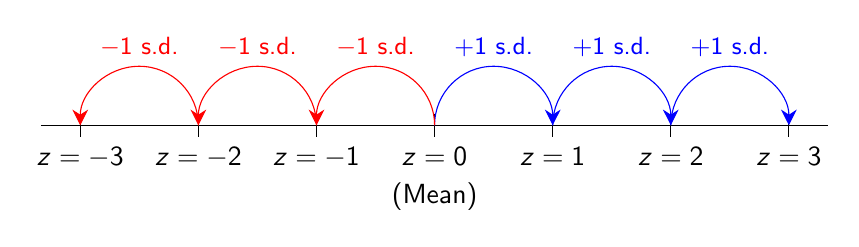
\begin{tikzpicture} \tikzset{>={Stealth[width=2mm,length=2mm]}}
\draw (-5,0) -- (5,0);
\foreach \x in {-4.5,-3,...,4.5}
\draw (\x, 0.15) -- (\x, -0.15);
\node at (0,-0.15) [below] {$z=0$};
\node at (0,-0.6) [below] {(Mean)};
\node at (1.5,-0.15) [below] {$z=1$};
\draw [->,blue] (0,0) arc (180:0:0.75) node [above, midway] {\small$+1\text{ s.d.}$};
\node at (3,-0.15) [below] {$z=2$};
\draw [->,blue] (1.5,0) arc (180:0:0.75) node [above, midway] {\small$+1\text{ s.d.}$};
\node at (4.5,-0.15) [below] {$z=3$};
\draw [->, blue] (3,0) arc (180:0:0.75) node [above, midway] {\small$+1\text{ s.d.}$};
\node at (-1.5,-0.15) [below] {$z=-1$};
\draw [->, red] (0,0) arc (0:180:0.75) node [above, midway] {\small$-1\text{ s.d.}$};
\node at (-3,-0.15) [below] {$z=-2$};
\draw [->, red] (-1.5,0) arc (0:180:0.75) node [above, midway] {\small$-1\text{ s.d.}$};
\node at (-4.5,-0.15) [below] {$z=-3$};
\draw [->, red] (-3,0) arc (0:180:0.75) node [above, midway] {\small$-1\text{ s.d.}$};
\end{tikzpicture}
\end{center}

\[z = \frac{x-\mu}{\sigma}\]	
\vspace{0.25in}

\begin{itemize}
    \item Can compare two different data sets that use different scales of measurement.
    \item ``Usual" data values have z-scores between $-2$ and 2.
\end{itemize}
\vspace{0.5in}

\begin{example}
The mean SAT score is 1059 with a standard deviation of 210; meanwhile the mean ACT score is 21 with a standard deviation of 5.4. A student takes both tests and receives a 1350 on the SAT and a 29 on the ACT. On which test did the student score better?
\end{example}

\newpage 

\subsection*{Percentiles}

\begin{tcolorbox}[colframe=green!20!black, colback = green!30!white,title=\textbf{Percentile}]
A \textbf{percentile} is a measure of location that divide a set of \emph{ordered} data into 100 groups with about 1\% of the values in each group.
\end{tcolorbox}

\vspace{0.25in}

\begin{tcolorbox}[colframe=green!20!black, colback = green!30!white,title=\textbf{Percentile Score}]
A \textbf{percentile score} is the percent of data values less than a given value. (\emph{Note}: this is \underline{not} the same as percentage).
\end{tcolorbox}
\vspace{1in}

\begin{example}
Explain the difference between getting 90\% on a test and scoring in the 90th percentile on that test.
\end{example}
\vspace{1.5in}

\emph{Note:} When working with percentiles, it is important to know whether or not the data value in question is included in the calculation.
\vspace{1in}

\begin{example}
Determine the percentile score value for the test score of 85 in the following data set. Only include values that are less than 85 in your calculation.
\begin{center}
    74, 74, 76, 77, 83, 85, 85, 90, 93, 94, 97, 98
\end{center}
\end{example}

\vfill 

\begin{example}
Determine the percentile score for 85 when you include values less than \emph{or equal to} 85.
\end{example}

\vfill 
\newpage 

\subsection*{Five-Number Summary}

\begin{tcolorbox}[colframe=green!20!black, colback = green!30!white,title=\textbf{Quartiles}]
\textbf{Quartiles} are values that divide a data set into 4 groups, with each group holding 25\% of the data.
\end{tcolorbox}
\vspace{8pt}	
\begin{center}
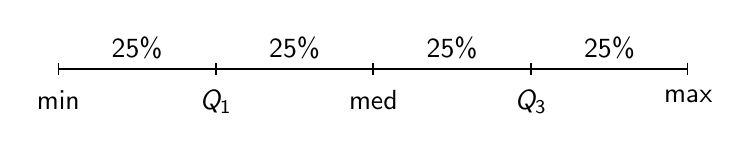
\begin{tikzpicture}
\coordinate (A) at (0,0);
\coordinate (B) at (2,0);
\coordinate (C) at (4,0);
\coordinate (D) at (6,0);
\coordinate (E) at (8,0);
\draw[|-|] (A) node [below, yshift=-0.15cm] {min} -- (B) node [midway, above] {25\%};
\draw[|-|] (B) node [below, yshift=-0.15cm] {$Q_1$} -- (C) node [midway, above] {25\%};
\draw[|-|] (C) node [below, yshift=-0.15cm] {med} -- (D) node [midway, above] {25\%};
\draw[|-|] (D) node [below, yshift=-0.15cm] {$Q_3$} -- (E) node [midway, above] {25\%};
\node at (E) [below, yshift=-0.15cm] {max};
\end{tikzpicture}
\end{center}
\vspace{8pt} 
$Q_1$ is called the first (a.k.a. \textit{lower}) quartile and $Q_3$ is called the third (a.k.a. \textit{upper}) quartile.

\vspace{1in}

\begin{tcolorbox}[colframe=green!20!black, colback = green!30!white,title=\textbf{Five-Number Summary}]
The \textbf{five-number summary} are the following values: 
\begin{center}
Minimum, $Q_1$, Median, $Q_3$, Maximum
\end{center}
\end{tcolorbox}
\vspace{1in}	

\begin{example}
Find the five-number summary of the following data set:
\begin{center}
    1, 2, 2, 4, 5, 7, 11, 15, 15, 18, 44
\end{center}
\end{example}

\vfill 
\newpage 

\subsubsection*{Detecting Outliers}

\begin{tcolorbox}[colframe=green!20!black, colback = green!30!white,title=\textbf{Outliers}]
An outlier is an extreme data value in a dataset.
\end{tcolorbox}
\vspace{8pt} 

We can use the five-number summary to detect outliers.	

\vspace{1in}

\begin{tcolorbox}[colframe=green!20!black, colback = green!30!white,title=\textbf{Interquartile Range}]
The \textbf{interquartile range} can be found by subtracting $Q_1$ from $Q_3$:
\[ \text{IQR} = Q_3 - Q_1 \]
\end{tcolorbox}

\vspace{1in}

The {\color{blue}\textbf{lower fence}} is
\[Q_1 - 1.5(\mathrm{IQR}) \]
and the {\color{blue}\textbf{upper fence} is}
\[Q_3 + 1.5(\mathrm{IQR}) \]

\vspace{0.5in}

A data value is an {\color{red}\textbf{outlier}} if it is less than the lower fence or more than the upper fence.

\vspace{2in}

\begin{example}
Calculate the lower and upper fences of the previous example's data set and use it to find any outliers.
\end{example}

\newpage


\subsection*{Box Plots}

\begin{tcolorbox}[colframe=green!20!black, colback = green!30!white,title=\textbf{Boxplot}]
A \textbf{box plot} (a.k.a. box-and-whisker plot) is a visual display of the five-number summary. 
\end{tcolorbox}
\vspace{8pt}	
\begin{center}
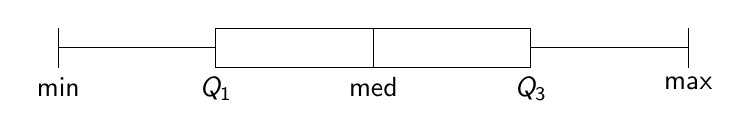
\begin{tikzpicture}
\draw (0,0.25) -- (0,-0.25) node [below] {min};
\draw (2,0.25) -- (2,-0.25) node [below] {$Q_1$};
\draw (4,0.25) -- (4,-0.25) node [below] {med};
\draw (6,0.25) -- (6,-0.25) node [below] {$Q_3$};
\draw (8,0.25) -- (8,-0.25) node [below] {max};
\draw (2,-0.25) rectangle (6,0.25);
\draw (0,0) -- (2,0);
\draw (6,0) -- (8,0);
\end{tikzpicture}
\end{center}

\vspace{1.75in}

\begin{example}
Create a box plot for the data set
\begin{center}
    1, 2, 2, 4, 5, 7, 11, 15, 15, 18, 44
\end{center}
\end{example}

\vfill 

\subsubsection*{Modified Box Plot}

\begin{itemize}
    \item Outliers are shown with symbols such as stars or points.
    \item Whiskers are drawn out to the points in the data set that are {\color{blue}\textbf{not}} considered outliers.
\end{itemize}

\vspace{0.25in}

\begin{center}
    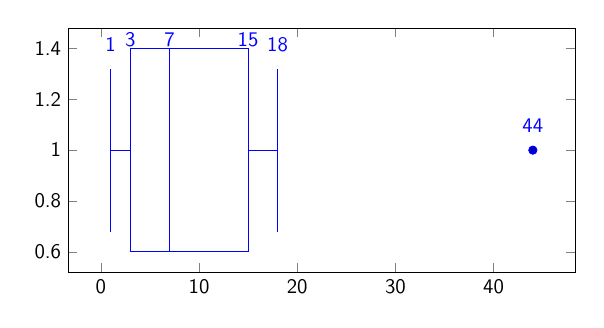
\begin{tikzpicture}[scale=0.75]
\begin{axis}[width=4in, height=2.25in]
\addplot+ [
boxplot prepared={
lower whisker=1,
lower quartile=3,
median=7,
upper quartile=15,
upper whisker=18,
},
] table [row sep=\\,y index=0] {
data\\ 44\\
}
[above]
node at
(boxplot box cs: \boxplotvalue{lower whisker},0.95)
{\pgfmathprintnumber{\boxplotvalue{lower whisker}}}
node at
(boxplot box cs: \boxplotvalue{lower quartile},0.975)
{\pgfmathprintnumber{\boxplotvalue{lower quartile}}}
node at
(boxplot box cs: \boxplotvalue{median},0.975)
{\pgfmathprintnumber{\boxplotvalue{median}}}
node at
(boxplot box cs: \boxplotvalue{upper quartile},0.975)
{\pgfmathprintnumber{\boxplotvalue{upper quartile}}}
node at
(boxplot box cs: \boxplotvalue{upper whisker},0.95)
{\pgfmathprintnumber{\boxplotvalue{upper whisker}}}
node at (boxplot box cs: 44,0.55) {44}
;
\end{axis}
\end{tikzpicture}
\end{center}
	
\vspace{1in}

\end{document}
